\documentclass[10pt,letterpaper]{article}
\usepackage[utf8]{inputenc}
\usepackage[english]{babel}
\usepackage{amsmath}
\usepackage{amsfonts}
\usepackage{amssymb}
\usepackage{graphicx}
\usepackage[left=2cm,right=2cm,top=2cm,bottom=2cm]{geometry}

\usepackage{pgfplots}
\pgfplotsset{compat=1.8}
\def\octavenominaldatam{data/data_1_voltagem.data}
\def\octavenominaldataa{data/data_1_voltagea.data}

\usepackage[]{mcode}

\begin{document}

\title{On the existence and linear approximation of the power flow solution\\
in power distribution networks -- Numerical analysis}
\author{Saverio Bolognani and Sandro Zampieri}

\maketitle

\begin{abstract}
This technical note reports an extensive numerical analysis of the approximate power flow method proposed in the paper by S. Bolognani and S. Zampieri, \textit{``On the existence and linear approximation of the power flow solution in power distribution networks''} \cite{Bolognani_powerflow}. Simulations are based on a modified version of the IEEE 123 test feeder. Different variations of the testbed have then been considered, in order to assess the performance of the approximate method for a range of practical cases. The technical details of the simulations, together with the simulation results and their interpretation, are included in this document. The Matlab / GNU Octave \cite{octave} and Matpower \cite{Zimmerman2011} code used in the simulations is available online \cite{github_approx-pf}.
\end{abstract}

\begin{figure}
\centering
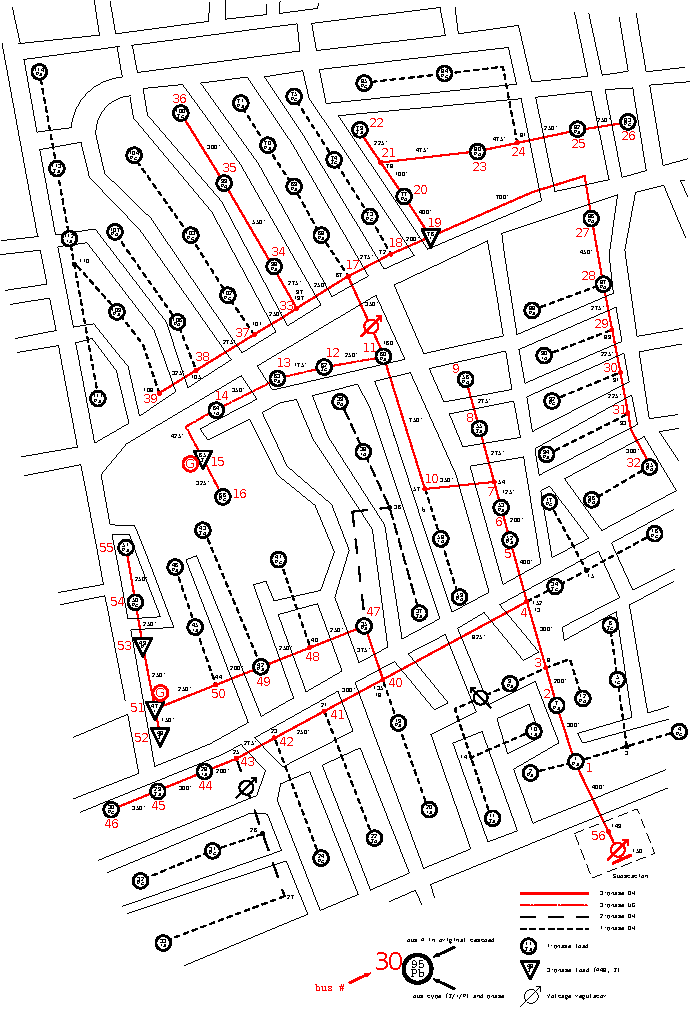
\includegraphics[height=\textheight]{ieee123}
\end{figure}

\section{Introduction}
\label{sec:intro}

The testbed used in these simulations has been obtained as a modification of the IEEE 123 Test Feeder \cite{Kersting2001,ieeetestfeeders}.
The following modifications have been introduced.
\begin{itemize}
\item Only the three-phase overhead lines and underground cables are considered. The resulting topology is illustrated in Section~\ref{sec:topology}.
\item Lines are assumed symmetric. Their line impedance is reported in Section~\ref{sec:topology}. 
\item Loads are assumed balanced and are modeled as PQ buses. All loads are located, as spot loads, at the point where their single phase feeder departs from the three phase feeder.
\item Shunt capacitors are assumed balanced.
\item Switches are in their normal position.
\item Voltage regulators are modeled as ideal transformers with variable tap position.
\item The tap changer at the substation is modeled as a slack node with variable voltage reference.
\item Microgenerators are connected at bus 15 and 51, and can be operated as a PV bus.
\end{itemize}

The modified testbed is available online as a MatPower case file \cite{github_approx-pf}.
This source code is distributed in the hope that it will be useful, but without any warranty. We do request that publications in which this testbed is adopted, explicitly acknowledge that fact by citing the original paper \cite{Bolognani_powerflow}.

\section{Grid topology}
\label{sec:topology}

The topology of the modified testbed is represented in the attached figure, where the original bus numbers from the IEEE 123 test feeder are also reported.
The network is radial, contains 56 nodes, and its segments are either three-phase overhead lines (OH) or three-phase underground cables (UG), with the following impedances. Distances (in yards) are reported in the attached figure, and corresponds to the distances in the original IEEE 123 testbed.

\noindent Three-phase impedance $Z_\text{OH}^{3\phi}$ in $\Omega/\text{mile}$:
$$
\begin{bmatrix}
0.46190 + 1.0638j 	& 0.15583 + 0.43673j 	& 0.15583 + 0.43673j \\
  					& 0.46190 + 1.0638j		& 0.15583 + 0.43673j \\
					&						& 0.46190 + 1.0638j
\end{bmatrix}
$$
Positive sequence impedance:
$$
Z_\text{OH} = 0.30607 + 0.62707j \ \text{[$\Omega$/mile]}
$$

\noindent Three-phase shunt admittance $Y_\text{OH}^{3\phi}$ in $\mu$ S/mile:
$$
\begin{bmatrix}
5.6848j 	& -1.2315j 	& -1.2315j \\
  					& 5.6848j		& -1.2315j \\
					&						& 5.6848j
\end{bmatrix}
$$
Positive sequence shunt admittance:
$$
Y_\text{OH} = 6.9163j \ \text{[$\mu$S/mile]}
$$


Three-phase impedance $Z_\text{UG}^{3\phi}$ in $\Omega/\text{mile}$:
$$
\begin{bmatrix}
1.5249 + 0.74013j	& 0.51067 + 0.25690j	& 0.51067 + 0.25690j \\
					& 1.5249 + 0.74013j	& 0.51067 + 0.25690j \\
					&						& 1.5249 + 0.74013j
\end{bmatrix}
$$
Positive sequence impedance:
$$
Z_\text{UG} =  1.01423 + 0.48323j \ \text{[$\Omega$/mile]}
$$

Three-phase shunt admittance $Y_\text{UG}^{3\phi}$ in $\mu$ S/mile:
$$
\begin{bmatrix}
67.2242j 	&  	&  \\
  					& 67.2242j		&  \\
					&						& 67.2242j
\end{bmatrix}
$$
Positive sequence shunt admittance:
$$
Y_\text{UG} = 67.2242j \ \text{[$\mu$S/mile]}
$$

%Simulations showed that, in this testbed, the shunt admittance of both the overhead lines and of the underground cables, is negligible. As discussed in \cite{Bolognani_powerflow}, the model can be seamlessly extended to the case of non-zero shunt admittances (see \ref{sec:scenario4} for a practical implementation).



%\lstinputlisting{../matpower4.1/case_ieee123.m}

\section{Simulations}

The following scenarios have been considered. 
\begin{enumerate}
\item \textbf{Nominal scenario} -- the nominal scenario with no shunt capacitor, nominal tap position at the voltage regulator, nominal tap position at the PCC, no voltage regulation at the microgenerator, total load and load distribution as in the original IEEE 123 test feeder (but balanced on the three phases). All the following scenarios depart from the nominal scenario as detailed hereafter.
\item \textbf{Uniform overload} -- the load of all the PQ buses is increased proportionally.
\item \textbf{Lumped overload} -- the load of one bus is increased.
\item \textbf{Shunt capacitor} -- shunt capacitors are connected for static voltage regulation.
\item \textbf{Voltage regulation} -- the voltage regulator is operated at a different tap position.
\item \textbf{Tap changer} -- the tap changer at the PCC is operated at a different tap position.
\item \textbf{PV buses} -- two voltage-regulated microgenerators are connected to the grid.
\item \textbf{High R/X ratio} -- all lines are replaced by underground cables.
\end{enumerate}

In the following, each one of these scenarios has been detailed, and the approximate power flow solution proposed in \cite{Bolognani_powerflow} has been plotted in \textbf{\color{red}red}, together with the solution returned by the MatPower nonlinear power flow solver. The nominal scenario is always plotted, as a reference, in \textbf{black}.

For each scenario, the absolute and relative errors in both voltage magnitude and angles are reported.
Relative errors are computed with respect to the bus voltage drop and to the bus angle (compared to the PCC), respectively.

% 1) nominal scenario
% 2) uniform overload
% 3) lumped overload
% 4) shunt capacitors
% 5) voltage regulation
% 6) tap changer
% 7) PV buses
% 8) High R/X ratio

\subsection{Nominal scenario}

The nominal scenario corresponds to the testbed adopted for the numerical experiments in the original paper \cite{Bolognani_powerflow}. As illustrated in the following figure, the approximation error is uniformly small across the grid, both in the voltage magnitudes and in the voltage angles.

\begin{verbatim}
Voltage absolute error [p.u.]:  0.004117 (avg.), 0.005621 (max)
Voltage relative error [%]:     7.886479 (avg.), 8.453902 (max)
Angle absolute error [p.u.]:    0.009687 (avg.), 0.017804 (max)
Angle relative error [%]:       0.437210 (avg.), 0.660915 (max)
\end{verbatim}

\begin{figure}
\begin{flushright}

\begin{tikzpicture}
[
	xscale	= 1,	% to scale horizontally everything but the text
	yscale	= 1,	% to scale vertically everything but the text
]
	%
	%
	%
	%
	%%%%%%%%%%%%%%%%%%%%%%%%%%%%%%%%%%%%%%%%%%%%%%%%%%%%%%%%%%%%%%%%%%%%%%
	%
	%
	\begin{axis}
	[
	footnotesize,
		xmode					= linear, 
		ymode					= linear,
%		enlarge x limits		= 0.5,
		width					= 170mm,
		height					= 50mm,
		%
		xmin					= 0,
		xmax					= 56,
%		ymin					= 0,
		ymax					= 1.02,
		%
%		xlabel					= {bus},
%		xlabel near ticks,
		%
		xtick					= {1, 55},
		xticklabels				= {bus 1, 55},
%		xmajorgrids,
		%
		ylabel					= {\footnotesize voltage magnitude [p.u.]},
		ylabel near ticks,
		%
%		ytick					= {0, 0.2, ..., 1},
%		yticklabels				= {0, 0.2, ..., 1},
%		ymajorgrids,
		%
		legend pos				= north east,
		legend columns			= 2,
		legend entries			= {exact solution $\ \ $, approximate model},
		legend cell align		= left,
		legend style			= {draw = none},
		%
		title style				= { align = center },
%		title					= {Voltage magnitude},
		%
%		axis background/.style	= {fill = black!05!white},
	]
		%
		% --------------------------------------------------------------
		\addplot
		[
			const plot,
			draw			= none,
			only marks,
			mark			= o,
			mark size		= 2pt,
		]
		table
		[
			x=bus,
			y=real,
		]
		{\octavenominaldatam};
		%
		% --------------------------------------------------------------
		\addplot
		[
			const plot,
			draw			= none,
			only marks,
			mark			= *,
			mark size		= 1pt,
		]
		table
		[
			x=bus,
			y=appr,
		]
		{\octavenominaldatam};
		%
		%
	\end{axis}
	%
\end{tikzpicture}


\begin{tikzpicture}
[
	xscale	= 1,	% to scale horizontally everything but the text
	yscale	= 1,	% to scale vertically everything but the text
]	
	%
	\begin{axis}
	[
	footnotesize,
		xmode					= linear, 
		ymode					= linear,
%		enlarge x limits		= 0.5,
		width					= 170mm,
		height					= 50mm,
		%
		xmin					= 0,
		xmax					= 56,
%		ymin					= 0,
		ymax					= 1,
		%
%		xlabel					= {bus},
%		xlabel near ticks,
		%
		xtick					= {1, 55},
		xticklabels				= {bus 1, 55},
%		xmajorgrids,
		%
		ylabel					= {\footnotesize voltage angle [deg]},
		ylabel near ticks,
		%
%		ytick					= {0, 0.2, ..., 1},
%		yticklabels				= {0, 0.2, ..., 1},
%		ymajorgrids,
		%
		legend pos				= north east,
		legend columns			= 2,
		legend entries			= {exact solution $\ \ $, approximate model},
		legend cell align		= left,
		legend style			= {draw = none},
		%
		title style				= { align = center },
%		title					= {Voltage magnitude},
		%
%		axis background/.style	= {fill = black!05!white},
	]
		%
		% --------------------------------------------------------------
		\addplot
		[
			const plot,
			draw			= none,
			only marks,
			mark			= o,
			mark size		= 2pt,
		]
		table
		[
			x=bus,
			y=real,
		]
		{\octavenominaldataa};
		%
		% --------------------------------------------------------------
		\addplot
		[
			const plot,
			draw			= none,
			only marks,
			mark			= *,
			mark size		= 1pt,
		]
		table
		[
			x=bus,
			y=appr,
		]
		{\octavenominaldataa};
		%
	\end{axis}
\end{tikzpicture}



\end{flushright}
\end{figure}

\subsection{Uniform overload}

In this scenario, the power demand of all buses has been doubled, in order to represent a case of relative overload of the power distribution grid. As illustrated in the following figure, for larger voltage drops (red), the approximation error increases compared to the nominal case (black), especially in the voltage magnitude.

\begin{verbatim}
Voltage absolute error [p.u.]:  0.019062 (avg.), 0.026102 (max)
Voltage relative error [%]:     16.718665 (avg.), 17.937571 (max)
Angle absolute error [p.u.]:    0.099920 (avg.), 0.178197 (max)
Angle relative error [%]:       2.088087 (avg.), 3.023680 (max)
\end{verbatim}

\def\octavedatam{data/data_2_voltagem.data}
\def\octavedataa{data/data_2_voltagea.data}
\documentclass{standalone}

%\renewcommand\familydefault{\sfdefault}

%\usepackage[cmex10]{amsmath}
\usepackage{amsfonts}
\usepackage{amssymb}
\usepackage{amsthm}
%\usepackage[T1]{fontenc}

\usepackage{pgfplots}
\pgfplotsset{compat=1.8}

\def\octavedata{data_paper_voltagem.data}

\begin{document}


\begin{tikzpicture}
[
	xscale	= 1,	% to scale horizontally everything but the text
	yscale	= 1,	% to scale vertically everything but the text
]
	%
	\begin{axis}
	[
	footnotesize,
		xmode					= linear, 
		ymode					= linear,
%		enlarge x limits		= 0.5,
		width					= 170mm,
		height					= 53mm,
		%
		xmin					= 0,
		xmax					= 56,
		ymin					= 0.57,
		ymax					= 1.03,
		%
%		xlabel					= {bus},
%		xlabel near ticks,
		%
		xtick					= {1, 55},
		xticklabels				= {bus 1, bus 55},
%		xmajorgrids,
		%
		ylabel					= {\footnotesize voltage magnitude $|v_h|$},
		ylabel near ticks,
		%
%		ytick					= {0, 0.2, ..., 1},
%		yticklabels				= {0, 0.2, ..., 1},
		ymajorgrids,
		grid style={dotted,gray},
		%
		legend pos				= south west,
		legend columns			= 1,
		legend entries			= {~exact solution, ~approximate model},
		legend cell align		= left,
		legend style			= {draw = none},
		%
		title style				= { align = center },
%		title					= {Voltage magnitude},
		%
%		axis background/.style	= {fill = black!05!white},
	]
		%
		% --------------------------------------------------------------
		\addplot
		[
			const plot,
%			dashed,
			draw			= none,
			only marks,
%			line width		= 1,
%			opacity			= 1,
			mark			= o,
			mark size		= 2pt,
		]
		table
		[
			x=bus,
			y=real,
		]
		{\octavedata};
%		\errorband[red, opacity=0.3]{data_voltagem.data}{0}{3}{4};
		%
		% --------------------------------------------------------------
		\addplot
		[
			const plot,
%			solid,
			draw			= none,
			only marks,
%			line width		= 1,
%			opacity			= 0.8,
			mark			= *,
			mark size		= 1pt,
		]
		table
		[
			x=bus,
			y=appr,
		]
		{\octavedata};
		%
		% --------------------------------------------------------------
		\addplot
		[
			%jump mark mid,
			%const plot,
			dashed,
			draw			= black,
%			line width		= 1,
			opacity			= 0.8,
			mark			= none,
		]
		table
		[
			x=bus,
			y=min1,
		]
		{\octavedata};
		%
		% --------------------------------------------------------------
		\addplot
		[
			%jump mark mid,
			dashed,
			draw			= black,
%			line width		= 1,
			opacity			= 0.8,
			mark			= none,
		]
		table
		[
			x=bus,
			y=max1,
		]
		{\octavedata};
		% --------------------------------------------------------------
		\addplot
		[
			%jump mark mid,
			%const plot,
			solid,
			draw			= black,
%			line width		= 1,
			opacity			= 0.8,
			mark			= none,
		]
		table
		[
			x=bus,
			y=min2,
		]
		{\octavedata};
		%
		% --------------------------------------------------------------
		\addplot
		[
			%jump mark mid,
			solid,
			draw			= black,
%			line width		= 1,
			opacity			= 0.8,
			mark			= none,
		]
		table
		[
			x=bus,
			y=max2,
		]
		{\octavedata};
		%
	\end{axis}
	%
\end{tikzpicture}



\end{document}

\subsection{Lumped overload}

In this scenario, the power demand of bus 32 has been increased to $2$ MW and $1$ MVAR. This significant lumped overload of the grid produces a localized drop in the voltage profile, which is also present in the approximate power flow solution. Also in this case, the overload condition slightly deteriorates the quality of the approximation.

\begin{verbatim}
Voltage absolute error [p.u.]:  0.019669 (avg.), 0.037333 (max)
Voltage relative error [%]:     18.986580 (avg.), 21.593179 (max)
Angle absolute error [p.u.]:    0.099379 (avg.), 0.311149 (max)
Angle relative error [%]:       2.119236 (avg.), 4.265142 (max)
\end{verbatim}

\def\octavedatam{data/data_3_voltagem.data}
\def\octavedataa{data/data_3_voltagea.data}
\begin{flushright}

\begin{tikzpicture}
[
	xscale	= 1,	% to scale horizontally everything but the text
	yscale	= 1,	% to scale vertically everything but the text
]
	%
	%
	%
	%
	%%%%%%%%%%%%%%%%%%%%%%%%%%%%%%%%%%%%%%%%%%%%%%%%%%%%%%%%%%%%%%%%%%%%%%
	%
	%
	\begin{axis}
	[
	footnotesize,
		xmode					= linear, 
		ymode					= linear,
%		enlarge x limits		= 0.5,
		width					= 170mm,
		height					= 50mm,
		%
		xmin					= 0,
		xmax					= 56,
%		ymin					= 0,
		ymax					= 1.02,
		%
%		xlabel					= {bus},
%		xlabel near ticks,
		%
		xtick					= {1, 55, 32},
		xticklabels				= {bus 1, 55, 32},
%		xmajorgrids,
		%
		ylabel					= {\footnotesize voltage magnitude [p.u.]},
		ylabel near ticks,
		%
%		ytick					= {0, 0.2, ..., 1},
%		yticklabels				= {0, 0.2, ..., 1},
%		ymajorgrids,
		%
		legend pos				= north east,
		legend columns			= 2,
		legend entries			= {exact solution $\ \ $, approximate model},
		legend cell align		= left,
		legend style			= {draw = none},
		%
		title style				= { align = center },
%		title					= {Voltage magnitude},
		%
%		axis background/.style	= {fill = black!05!white},
	]
		%
		% --------------------------------------------------------------
		\addplot
		[
			const plot,
			draw			= none,
			only marks,
			mark			= o,
			mark size		= 2pt,
		]
		table
		[
			x=bus,
			y=real,
		]
		{\octavenominaldatam};
		%
		% --------------------------------------------------------------
		\addplot
		[
			const plot,
			draw			= none,
			only marks,
			mark			= *,
			mark size		= 1pt,
		]
		table
		[
			x=bus,
			y=appr,
		]
		{\octavenominaldatam};
		%
		% --------------------------------------------------------------
		\addplot
		[
			const plot,
			draw			= none,
			only marks,
			mark			= o,
			mark size		= 2pt,
			color			= red,
		]
		table
		[
			x=bus,
			y=real,
		]
		{\octavedatam};
		%
		% --------------------------------------------------------------
		\addplot
		[
			const plot,
			draw			= none,
			only marks,
			mark			= *,
			mark size		= 1pt,
			color			= red,
		]
		table
		[
			x=bus,
			y=appr,
		]
		{\octavedatam};
		%
		% --------------------------------------------------------------		
		%
	\end{axis}
	%
\end{tikzpicture}


\begin{tikzpicture}
[
	xscale	= 1,	% to scale horizontally everything but the text
	yscale	= 1,	% to scale vertically everything but the text
]	
	%
	\begin{axis}
	[
	footnotesize,
		xmode					= linear, 
		ymode					= linear,
%		enlarge x limits		= 0.5,
		width					= 170mm,
		height					= 50mm,
		%
		xmin					= 0,
		xmax					= 56,
%		ymin					= 0,
		ymax					= 1,
		%
%		xlabel					= {bus},
%		xlabel near ticks,
		%
		xtick					= {1, 55},
		xticklabels				= {bus 1, bus 55},
%		xmajorgrids,
		%
		ylabel					= {\footnotesize voltage angle [deg]},
		ylabel near ticks,
		%
%		ytick					= {0, 0.2, ..., 1},
%		yticklabels				= {0, 0.2, ..., 1},
%		ymajorgrids,
		%
		legend pos				= north east,
		legend columns			= 2,
		legend entries			= {exact solution $\ \ $, approximate model},
		legend cell align		= left,
		legend style			= {draw = none},
		%
		title style				= { align = center },
%		title					= {Voltage magnitude},
		%
%		axis background/.style	= {fill = black!05!white},
	]
		%
		% --------------------------------------------------------------
		\addplot
		[
			const plot,
			draw			= none,
			only marks,
			mark			= o,
			mark size		= 2pt,
		]
		table
		[
			x=bus,
			y=real,
		]
		{\octavenominaldataa};
		%
		% --------------------------------------------------------------
		\addplot
		[
			const plot,
			draw			= none,
			only marks,
			mark			= *,
			mark size		= 1pt,
		]
		table
		[
			x=bus,
			y=appr,
		]
		{\octavenominaldataa};
		%
		% --------------------------------------------------------------
		\addplot
		[
			const plot,
			draw			= none,
			only marks,
			mark			= o,
			mark size		= 2pt,
			color			= red,
		]
		table
		[
			x=bus,
			y=real,
		]
		{\octavedataa};
		%
		% --------------------------------------------------------------
		\addplot
		[
			const plot,
			draw			= none,
			only marks,
			mark			= *,
			mark size		= 1pt,
			color			= red,
		]
		table
		[
			x=bus,
			y=appr,
		]
		{\octavedataa};
		%
		% --------------------------------------------------------------		
		%
	\end{axis}
\end{tikzpicture}



\end{flushright}

\subsection{Shunt capacitor}
\label{sec:scenario4}

In this scenario, shunt capacitors have been connected to buses 26 (600 KVAR), 28 (50 KVAR), 29 (50 KVAR), 30 (50 KVAR), according to what is suggested in the original testbed, in order to support the voltage. 

\begin{verbatim}
Voltage absolute error [p.u.]:  0.005215 (avg.), 0.008138 (max)
Voltage relative error [%]:     13.373612 (avg.), 21.329141 (max)
Angle absolute error [p.u.]:    0.028870 (avg.), 0.049064 (max)
Angle relative error [%]:       1.244363 (avg.), 1.860290 (max)
\end{verbatim}

\def\octavedatam{data/data_4_voltagem.data}
\def\octavedataa{data/data_4_voltagea.data}
\begin{flushright}

\begin{tikzpicture}
[
	xscale	= 1,	% to scale horizontally everything but the text
	yscale	= 1,	% to scale vertically everything but the text
]
	%
	%
	%
	%
	%%%%%%%%%%%%%%%%%%%%%%%%%%%%%%%%%%%%%%%%%%%%%%%%%%%%%%%%%%%%%%%%%%%%%%
	%
	%
	\begin{axis}
	[
	footnotesize,
		xmode					= linear, 
		ymode					= linear,
%		enlarge x limits		= 0.5,
		width					= 170mm,
		height					= 50mm,
		%
		xmin					= 0,
		xmax					= 56,
%		ymin					= 0,
		ymax					= 1.02,
		%
%		xlabel					= {bus},
%		xlabel near ticks,
		%
		xtick					= {1, 55, 26, 28, 29, 30},
		xticklabels				= {bus 1, 55, \scriptsize 26, \scriptsize 28, \scriptsize 29, \scriptsize 30},
%		xmajorgrids,
		%
		ylabel					= {\footnotesize voltage magnitude [p.u.]},
		ylabel near ticks,
		%
%		ytick					= {0, 0.2, ..., 1},
%		yticklabels				= {0, 0.2, ..., 1},
%		ymajorgrids,
		%
		legend pos				= north east,
		legend columns			= 2,
		legend entries			= {exact solution $\ \ $, approximate model},
		legend cell align		= left,
		legend style			= {draw = none},
		%
		title style				= { align = center },
%		title					= {Voltage magnitude},
		%
%		axis background/.style	= {fill = black!05!white},
	]
		%
		% --------------------------------------------------------------
		\addplot
		[
			const plot,
			draw			= none,
			only marks,
			mark			= o,
			mark size		= 2pt,
		]
		table
		[
			x=bus,
			y=real,
		]
		{\octavenominaldatam};
		%
		% --------------------------------------------------------------
		\addplot
		[
			const plot,
			draw			= none,
			only marks,
			mark			= *,
			mark size		= 1pt,
		]
		table
		[
			x=bus,
			y=appr,
		]
		{\octavenominaldatam};
		%
		% --------------------------------------------------------------
		\addplot
		[
			const plot,
			draw			= none,
			only marks,
			mark			= o,
			mark size		= 2pt,
			color			= red,
		]
		table
		[
			x=bus,
			y=real,
		]
		{\octavedatam};
		%
		% --------------------------------------------------------------
		\addplot
		[
			const plot,
			draw			= none,
			only marks,
			mark			= *,
			mark size		= 1pt,
			color			= red,
		]
		table
		[
			x=bus,
			y=appr,
		]
		{\octavedatam};
		%
		% --------------------------------------------------------------		
		%
	\end{axis}
	%
\end{tikzpicture}


\begin{tikzpicture}
[
	xscale	= 1,	% to scale horizontally everything but the text
	yscale	= 1,	% to scale vertically everything but the text
]	
	%
	\begin{axis}
	[
	footnotesize,
		xmode					= linear, 
		ymode					= linear,
%		enlarge x limits		= 0.5,
		width					= 170mm,
		height					= 50mm,
		%
		xmin					= 0,
		xmax					= 56,
%		ymin					= 0,
		ymax					= 1,
		%
%		xlabel					= {bus},
%		xlabel near ticks,
		%
		xtick					= {1, 55, 26, 28, 29, 30},
		xticklabels				= {bus 1, 55, \scriptsize 26, \scriptsize 28, \scriptsize 29, \scriptsize 30},
%		xmajorgrids,
		%
		ylabel					= {\footnotesize voltage angle [deg]},
		ylabel near ticks,
		%
%		ytick					= {0, 0.2, ..., 1},
%		yticklabels				= {0, 0.2, ..., 1},
%		ymajorgrids,
		%
		legend pos				= north east,
		legend columns			= 2,
		legend entries			= {exact solution $\ \ $, approximate model},
		legend cell align		= left,
		legend style			= {draw = none},
		%
		title style				= { align = center },
%		title					= {Voltage magnitude},
		%
%		axis background/.style	= {fill = black!05!white},
	]
		%
		% --------------------------------------------------------------
		\addplot
		[
			const plot,
			draw			= none,
			only marks,
			mark			= o,
			mark size		= 2pt,
		]
		table
		[
			x=bus,
			y=real,
		]
		{\octavenominaldataa};
		%
		% --------------------------------------------------------------
		\addplot
		[
			const plot,
			draw			= none,
			only marks,
			mark			= *,
			mark size		= 1pt,
		]
		table
		[
			x=bus,
			y=appr,
		]
		{\octavenominaldataa};
		%
		% --------------------------------------------------------------
		\addplot
		[
			const plot,
			draw			= none,
			only marks,
			mark			= o,
			mark size		= 2pt,
			color			= red,
		]
		table
		[
			x=bus,
			y=real,
		]
		{\octavedataa};
		%
		% --------------------------------------------------------------
		\addplot
		[
			const plot,
			draw			= none,
			only marks,
			mark			= *,
			mark size		= 1pt,
			color			= red,
		]
		table
		[
			x=bus,
			y=appr,
		]
		{\octavedataa};
		%
		% --------------------------------------------------------------		
		%
	\end{axis}
\end{tikzpicture}



\end{flushright}

\subsection{Voltage regulation}

In this scenario, the voltage regulator that connects bus 11 with bus 17 is operated at a tap different from the nominal tap, obtaining a voltage ratio of 124/120. Because the voltage regulator is modeled as an ideal transformer, this device can be included in the model by proper scaling of the portion of the bus admittance matrix that involves the buses fed by the voltage regulator (buses 17 to 39).

\begin{verbatim}
Voltage absolute error [p.u.]:  0.003788 (avg.), 0.005004 (max)
Voltage relative error [%]:     10.341566 (avg.), 16.201909 (max)
Angle absolute error [p.u.]:    0.013116 (avg.), 0.037686 (max)
Angle relative error [%]:       0.568924 (avg.), 1.413201 (max)
\end{verbatim}

\def\octavedatam{data/data_5_voltagem.data}
\def\octavedataa{data/data_5_voltagea.data}
\begin{flushright}

\begin{tikzpicture}
[
	xscale	= 1,	% to scale horizontally everything but the text
	yscale	= 1,	% to scale vertically everything but the text
]
	%
	%
	%
	%
	%%%%%%%%%%%%%%%%%%%%%%%%%%%%%%%%%%%%%%%%%%%%%%%%%%%%%%%%%%%%%%%%%%%%%%
	%
	%
	\begin{axis}
	[
	footnotesize,
		xmode					= linear, 
		ymode					= linear,
%		enlarge x limits		= 0.5,
		width					= 170mm,
		height					= 50mm,
		%
		xmin					= 0,
		xmax					= 56,
%		ymin					= 0,
		ymax					= 1.02,
		%
%		xlabel					= {bus},
%		xlabel near ticks,
		%
		xtick					= {1, 55, 17, 39},
		xticklabels				= {bus 1, 55, 17, 39},
%		xmajorgrids,
		%
		ylabel					= {\footnotesize voltage magnitude [p.u.]},
		ylabel near ticks,
		%
%		ytick					= {0, 0.2, ..., 1},
%		yticklabels				= {0, 0.2, ..., 1},
%		ymajorgrids,
		%
		legend pos				= north east,
		legend columns			= 2,
		legend entries			= {exact solution $\ \ $, approximate model},
		legend cell align		= left,
		legend style			= {draw = none},
		%
		title style				= { align = center },
%		title					= {Voltage magnitude},
		%
%		axis background/.style	= {fill = black!05!white},
	]
		%
		% --------------------------------------------------------------
		\addplot
		[
			const plot,
			draw			= none,
			only marks,
			mark			= o,
			mark size		= 2pt,
		]
		table
		[
			x=bus,
			y=real,
		]
		{\octavenominaldatam};
		%
		% --------------------------------------------------------------
		\addplot
		[
			const plot,
			draw			= none,
			only marks,
			mark			= *,
			mark size		= 1pt,
		]
		table
		[
			x=bus,
			y=appr,
		]
		{\octavenominaldatam};
		%
		% --------------------------------------------------------------
		\addplot
		[
			const plot,
			draw			= none,
			only marks,
			mark			= o,
			mark size		= 2pt,
			color			= red,
		]
		table
		[
			x=bus,
			y=real,
		]
		{\octavedatam};
		%
		% --------------------------------------------------------------
		\addplot
		[
			const plot,
			draw			= none,
			only marks,
			mark			= *,
			mark size		= 1pt,
			color			= red,
		]
		table
		[
			x=bus,
			y=appr,
		]
		{\octavedatam};
		%
		% --------------------------------------------------------------		
		%
	\end{axis}
	%
\end{tikzpicture}


\begin{tikzpicture}
[
	xscale	= 1,	% to scale horizontally everything but the text
	yscale	= 1,	% to scale vertically everything but the text
]	
	%
	\begin{axis}
	[
	footnotesize,
		xmode					= linear, 
		ymode					= linear,
%		enlarge x limits		= 0.5,
		width					= 170mm,
		height					= 50mm,
		%
		xmin					= 0,
		xmax					= 56,
%		ymin					= 0,
		ymax					= 1,
		%
%		xlabel					= {bus},
%		xlabel near ticks,
		%
		xtick					= {1, 55, 17, 39},
		xticklabels				= {bus 1, 55, 17, 39},
%		xmajorgrids,
		%
		ylabel					= {\footnotesize voltage angle [deg]},
		ylabel near ticks,
		%
%		ytick					= {0, 0.2, ..., 1},
%		yticklabels				= {0, 0.2, ..., 1},
%		ymajorgrids,
		%
		legend pos				= north east,
		legend columns			= 2,
		legend entries			= {exact solution $\ \ $, approximate model},
		legend cell align		= left,
		legend style			= {draw = none},
		%
		title style				= { align = center },
%		title					= {Voltage magnitude},
		%
%		axis background/.style	= {fill = black!05!white},
	]
		%
		% --------------------------------------------------------------
		\addplot
		[
			const plot,
			draw			= none,
			only marks,
			mark			= o,
			mark size		= 2pt,
		]
		table
		[
			x=bus,
			y=real,
		]
		{\octavenominaldataa};
		%
		% --------------------------------------------------------------
		\addplot
		[
			const plot,
			draw			= none,
			only marks,
			mark			= *,
			mark size		= 1pt,
		]
		table
		[
			x=bus,
			y=appr,
		]
		{\octavenominaldataa};
		%
		% --------------------------------------------------------------
		\addplot
		[
			const plot,
			draw			= none,
			only marks,
			mark			= o,
			mark size		= 2pt,
			color			= red,
		]
		table
		[
			x=bus,
			y=real,
		]
		{\octavedataa};
		%
		% --------------------------------------------------------------
		\addplot
		[
			const plot,
			draw			= none,
			only marks,
			mark			= *,
			mark size		= 1pt,
			color			= red,
		]
		table
		[
			x=bus,
			y=appr,
		]
		{\octavedataa};
		%
		% --------------------------------------------------------------		
		%
	\end{axis}
\end{tikzpicture}



\end{flushright}

\subsection{Tap changer}

In this scenario, the tap changer at the PCC of the test feeder is operated at a tap different from the nominal tap, obtaining a secondary voltage of 124/120. 

\begin{verbatim}
Voltage absolute error [p.u.]:  0.003701 (avg.), 0.005053 (max)
Voltage relative error [%]:     7.362317 (avg.), 7.891349 (max)
Angle absolute error [p.u.]:    0.007903 (avg.), 0.014524 (max)
Angle relative error [%]:       0.382406 (avg.), 0.578529 (max)
\end{verbatim}

\def\octavedatam{data/data_6_voltagem.data}
\def\octavedataa{data/data_6_voltagea.data}
\begin{flushright}

\begin{tikzpicture}
[
	xscale	= 1,	% to scale horizontally everything but the text
	yscale	= 1,	% to scale vertically everything but the text
]
	%
	%
	%
	%
	%%%%%%%%%%%%%%%%%%%%%%%%%%%%%%%%%%%%%%%%%%%%%%%%%%%%%%%%%%%%%%%%%%%%%%
	%
	%
	\begin{axis}
	[
	footnotesize,
		xmode					= linear, 
		ymode					= linear,
%		enlarge x limits		= 0.5,
		width					= 170mm,
		height					= 50mm,
		%
		xmin					= 0,
		xmax					= 56,
%		ymin					= 0,
		ymax					= 1.03,
		%
%		xlabel					= {bus},
%		xlabel near ticks,
		%
		xtick					= {1, 55},
		xticklabels				= {bus 1, 55},
%		xmajorgrids,
		%
		ylabel					= {\footnotesize voltage magnitude [p.u.]},
		ylabel near ticks,
		%
%		ytick					= {0, 0.2, ..., 1},
%		yticklabels				= {0, 0.2, ..., 1},
%		ymajorgrids,
		%
		legend pos				= north east,
		legend columns			= 2,
		legend entries			= {exact solution $\ \ $, approximate model},
		legend cell align		= left,
		legend style			= {draw = none},
		%
		title style				= { align = center },
%		title					= {Voltage magnitude},
		%
%		axis background/.style	= {fill = black!05!white},
	]
		%
		% --------------------------------------------------------------
		\addplot
		[
			const plot,
			draw			= none,
			only marks,
			mark			= o,
			mark size		= 2pt,
		]
		table
		[
			x=bus,
			y=real,
		]
		{\octavenominaldatam};
		%
		% --------------------------------------------------------------
		\addplot
		[
			const plot,
			draw			= none,
			only marks,
			mark			= *,
			mark size		= 1pt,
		]
		table
		[
			x=bus,
			y=appr,
		]
		{\octavenominaldatam};
		%
		% --------------------------------------------------------------
		\addplot
		[
			const plot,
			draw			= none,
			only marks,
			mark			= o,
			mark size		= 2pt,
			color			= red,
		]
		table
		[
			x=bus,
			y=real,
		]
		{\octavedatam};
		%
		% --------------------------------------------------------------
		\addplot
		[
			const plot,
			draw			= none,
			only marks,
			mark			= *,
			mark size		= 1pt,
			color			= red,
		]
		table
		[
			x=bus,
			y=appr,
		]
		{\octavedatam};
		%
		% --------------------------------------------------------------		
		%
	\end{axis}
	%
\end{tikzpicture}


\begin{tikzpicture}
[
	xscale	= 1,	% to scale horizontally everything but the text
	yscale	= 1,	% to scale vertically everything but the text
]	
	%
	\begin{axis}
	[
	footnotesize,
		xmode					= linear, 
		ymode					= linear,
%		enlarge x limits		= 0.5,
		width					= 170mm,
		height					= 50mm,
		%
		xmin					= 0,
		xmax					= 56,
%		ymin					= 0,
		ymax					= 1,
		%
%		xlabel					= {bus},
%		xlabel near ticks,
		%
		xtick					= {1, 55},
		xticklabels				= {bus 1, bus 55},
%		xmajorgrids,
		%
		ylabel					= {\footnotesize voltage angle [deg]},
		ylabel near ticks,
		%
%		ytick					= {0, 0.2, ..., 1},
%		yticklabels				= {0, 0.2, ..., 1},
%		ymajorgrids,
		%
		legend pos				= north east,
		legend columns			= 2,
		legend entries			= {exact solution $\ \ $, approximate model},
		legend cell align		= left,
		legend style			= {draw = none},
		%
		title style				= { align = center },
%		title					= {Voltage magnitude},
		%
%		axis background/.style	= {fill = black!05!white},
	]
		%
		% --------------------------------------------------------------
		\addplot
		[
			const plot,
			draw			= none,
			only marks,
			mark			= o,
			mark size		= 2pt,
		]
		table
		[
			x=bus,
			y=real,
		]
		{\octavenominaldataa};
		%
		% --------------------------------------------------------------
		\addplot
		[
			const plot,
			draw			= none,
			only marks,
			mark			= *,
			mark size		= 1pt,
		]
		table
		[
			x=bus,
			y=appr,
		]
		{\octavenominaldataa};
		%
		% --------------------------------------------------------------
		\addplot
		[
			const plot,
			draw			= none,
			only marks,
			mark			= o,
			mark size		= 2pt,
			color			= red,
		]
		table
		[
			x=bus,
			y=real,
		]
		{\octavedataa};
		%
		% --------------------------------------------------------------
		\addplot
		[
			const plot,
			draw			= none,
			only marks,
			mark			= *,
			mark size		= 1pt,
			color			= red,
		]
		table
		[
			x=bus,
			y=appr,
		]
		{\octavedataa};
		%
		% --------------------------------------------------------------		
		%
	\end{axis}
\end{tikzpicture}



\end{flushright}

\subsection{PV buses}

In this scenario, the generator connected to bus 15 is voltage regulated, with a voltage reference of 1 p.u. 
%As described in the original paper \cite{Bolognani_powerflow}, the approximate model can be properly modified, so that the resulting model is linear in the power demands of the PQ buses, in the active power injection of the PV bus, and in the voltage reference of the PV bus.

\begin{verbatim}
Voltage absolute error [p.u.]:  0.000481 (avg.), 0.001404 (max)
Voltage relative error [%]:     Inf (avg.), Inf (max)
Angle absolute error [p.u.]:    0.155125 (avg.), 0.371735 (max)
Angle relative error [%]:       4.770471 (avg.), 7.440988 (max)
\end{verbatim}

\def\octavedatam{data/data_7_voltagem.data}
\def\octavedataa{data/data_7_voltagea.data}
\begin{flushright}

\begin{tikzpicture}
[
	xscale	= 1,	% to scale horizontally everything but the text
	yscale	= 1,	% to scale vertically everything but the text
]
	%
	%
	%
	%
	%%%%%%%%%%%%%%%%%%%%%%%%%%%%%%%%%%%%%%%%%%%%%%%%%%%%%%%%%%%%%%%%%%%%%%
	%
	%
	\begin{axis}
	[
	footnotesize,
		xmode					= linear, 
		ymode					= linear,
%		enlarge x limits		= 0.5,
		width					= 170mm,
		height					= 50mm,
		%
		xmin					= 0,
		xmax					= 56,
%		ymin					= 0,
		ymax					= 1.02,
		%
%		xlabel					= {bus},
%		xlabel near ticks,
		%
		xtick					= {1, 55, 15},
		xticklabels				= {bus 1, 55, 15},
%		xmajorgrids,
		%
		ylabel					= {\footnotesize voltage magnitude [p.u.]},
		ylabel near ticks,
		%
%		ytick					= {0, 0.2, ..., 1},
%		yticklabels				= {0, 0.2, ..., 1},
%		ymajorgrids,
		%
		legend pos				= north east,
		legend columns			= 2,
		legend entries			= {exact solution $\ \ $, approximate model},
		legend cell align		= left,
		legend style			= {draw = none},
		%
		title style				= { align = center },
%		title					= {Voltage magnitude},
		%
%		axis background/.style	= {fill = black!05!white},
	]
		%
		% --------------------------------------------------------------
		\addplot
		[
			const plot,
			draw			= none,
			only marks,
			mark			= o,
			mark size		= 2pt,
		]
		table
		[
			x=bus,
			y=real,
		]
		{\octavenominaldatam};
		%
		% --------------------------------------------------------------
		\addplot
		[
			const plot,
			draw			= none,
			only marks,
			mark			= *,
			mark size		= 1pt,
		]
		table
		[
			x=bus,
			y=appr,
		]
		{\octavenominaldatam};
		%
		% --------------------------------------------------------------
		\addplot
		[
			const plot,
			draw			= none,
			only marks,
			mark			= o,
			mark size		= 2pt,
			color			= red,
		]
		table
		[
			x=bus,
			y=real,
		]
		{\octavedatam};
		%
		% --------------------------------------------------------------
		\addplot
		[
			const plot,
			draw			= none,
			only marks,
			mark			= *,
			mark size		= 1pt,
			color			= red,
		]
		table
		[
			x=bus,
			y=appr,
		]
		{\octavedatam};
		%
		% --------------------------------------------------------------		
		%
	\end{axis}
	%
\end{tikzpicture}


\begin{tikzpicture}
[
	xscale	= 1,	% to scale horizontally everything but the text
	yscale	= 1,	% to scale vertically everything but the text
]	
	%
	\begin{axis}
	[
	footnotesize,
		xmode					= linear, 
		ymode					= linear,
%		enlarge x limits		= 0.5,
		width					= 170mm,
		height					= 50mm,
		%
		xmin					= 0,
		xmax					= 56,
%		ymin					= 0,
		ymax					= 1,
		%
%		xlabel					= {bus},
%		xlabel near ticks,
		%
		xtick					= {1, 55, 15},
		xticklabels				= {bus 1, 55, 15},
%		xmajorgrids,
		%
		ylabel					= {\footnotesize voltage angle [deg]},
		ylabel near ticks,
		%
%		ytick					= {0, 0.2, ..., 1},
%		yticklabels				= {0, 0.2, ..., 1},
%		ymajorgrids,
		%
		legend pos				= north east,
		legend columns			= 2,
		legend entries			= {exact solution $\ \ $, approximate model},
		legend cell align		= left,
		legend style			= {draw = none},
		%
		title style				= { align = center },
%		title					= {Voltage magnitude},
		%
%		axis background/.style	= {fill = black!05!white},
	]
		%
		% --------------------------------------------------------------
		\addplot
		[
			const plot,
			draw			= none,
			only marks,
			mark			= o,
			mark size		= 2pt,
		]
		table
		[
			x=bus,
			y=real,
		]
		{\octavenominaldataa};
		%
		% --------------------------------------------------------------
		\addplot
		[
			const plot,
			draw			= none,
			only marks,
			mark			= *,
			mark size		= 1pt,
		]
		table
		[
			x=bus,
			y=appr,
		]
		{\octavenominaldataa};
		%
		% --------------------------------------------------------------
		\addplot
		[
			const plot,
			draw			= none,
			only marks,
			mark			= o,
			mark size		= 2pt,
			color			= red,
		]
		table
		[
			x=bus,
			y=real,
		]
		{\octavedataa};
		%
		% --------------------------------------------------------------
		\addplot
		[
			const plot,
			draw			= none,
			only marks,
			mark			= *,
			mark size		= 1pt,
			color			= red,
		]
		table
		[
			x=bus,
			y=appr,
		]
		{\octavedataa};
		%
		% --------------------------------------------------------------		
		%
	\end{axis}
\end{tikzpicture}



\end{flushright}

\subsection{High R/X ratio}

In this scenario, all overhead lines in the testbed have been replaced by underground cables, exhibiting a larger R/X ratio. 
%As described in the original paper \cite{Bolognani_powerflow}, the approximate model can be properly modified, so that the resulting model is linear in the power demands of the PQ buses, in the active power injection of the PV bus, and in the voltage reference of the PV bus.

\begin{verbatim}
Voltage absolute error [p.u.]:  0.012174 (avg.), 0.016715 (max)
Voltage relative error [%]:     11.311448 (avg.), 12.057741 (max)
Angle absolute error [p.u.]:    0.005106 (avg.), 0.010107 (max)
Angle relative error [%]:       1.351258 (avg.), 2.574156 (max)

\end{verbatim}

\def\octavedatam{data/data_8_voltagem.data}
\def\octavedataa{data/data_8_voltagea.data}
\begin{flushright}

\begin{tikzpicture}
[
	xscale	= 1,	% to scale horizontally everything but the text
	yscale	= 1,	% to scale vertically everything but the text
]
	%
	%
	%
	%
	%%%%%%%%%%%%%%%%%%%%%%%%%%%%%%%%%%%%%%%%%%%%%%%%%%%%%%%%%%%%%%%%%%%%%%
	%
	%
	\begin{axis}
	[
	footnotesize,
		xmode					= linear, 
		ymode					= linear,
%		enlarge x limits		= 0.5,
		width					= 170mm,
		height					= 50mm,
		%
		xmin					= 0,
		xmax					= 56,
%		ymin					= 0,
		ymax					= 1.02,
		%
%		xlabel					= {bus},
%		xlabel near ticks,
		%
		xtick					= {1, 55},
		xticklabels				= {bus 1, 55},
%		xmajorgrids,
		%
		ylabel					= {\footnotesize voltage magnitude [p.u.]},
		ylabel near ticks,
		%
%		ytick					= {0, 0.2, ..., 1},
%		yticklabels				= {0, 0.2, ..., 1},
%		ymajorgrids,
		%
		legend pos				= north east,
		legend columns			= 2,
		legend entries			= {exact solution $\ \ $, approximate model},
		legend cell align		= left,
		legend style			= {draw = none},
		%
		title style				= { align = center },
%		title					= {Voltage magnitude},
		%
%		axis background/.style	= {fill = black!05!white},
	]
		%
		% --------------------------------------------------------------
		\addplot
		[
			const plot,
			draw			= none,
			only marks,
			mark			= o,
			mark size		= 2pt,
		]
		table
		[
			x=bus,
			y=real,
		]
		{\octavenominaldatam};
		%
		% --------------------------------------------------------------
		\addplot
		[
			const plot,
			draw			= none,
			only marks,
			mark			= *,
			mark size		= 1pt,
		]
		table
		[
			x=bus,
			y=appr,
		]
		{\octavenominaldatam};
		%
		% --------------------------------------------------------------
		\addplot
		[
			const plot,
			draw			= none,
			only marks,
			mark			= o,
			mark size		= 2pt,
			color			= red,
		]
		table
		[
			x=bus,
			y=real,
		]
		{\octavedatam};
		%
		% --------------------------------------------------------------
		\addplot
		[
			const plot,
			draw			= none,
			only marks,
			mark			= *,
			mark size		= 1pt,
			color			= red,
		]
		table
		[
			x=bus,
			y=appr,
		]
		{\octavedatam};
		%
		% --------------------------------------------------------------		
		%
	\end{axis}
	%
\end{tikzpicture}


\begin{tikzpicture}
[
	xscale	= 1,	% to scale horizontally everything but the text
	yscale	= 1,	% to scale vertically everything but the text
]	
	%
	\begin{axis}
	[
	footnotesize,
		xmode					= linear, 
		ymode					= linear,
%		enlarge x limits		= 0.5,
		width					= 170mm,
		height					= 50mm,
		%
		xmin					= 0,
		xmax					= 56,
%		ymin					= 0,
		ymax					= 1.5,
		%
%		xlabel					= {bus},
%		xlabel near ticks,
		%
		xtick					= {1, 55},
		xticklabels				= {bus 1, 55},
%		xmajorgrids,
		%
		ylabel					= {\footnotesize voltage angle [deg]},
		ylabel near ticks,
		%
%		ytick					= {0, 0.2, ..., 1},
%		yticklabels				= {0, 0.2, ..., 1},
%		ymajorgrids,
		%
		legend pos				= north east,
		legend columns			= 2,
		legend entries			= {exact solution $\ \ $, approximate model},
		legend cell align		= left,
		legend style			= {draw = none},
		%
		title style				= { align = center },
%		title					= {Voltage magnitude},
		%
%		axis background/.style	= {fill = black!05!white},
	]
		%
		% --------------------------------------------------------------
		\addplot
		[
			const plot,
			draw			= none,
			only marks,
			mark			= o,
			mark size		= 2pt,
		]
		table
		[
			x=bus,
			y=real,
		]
		{\octavenominaldataa};
		%
		% --------------------------------------------------------------
		\addplot
		[
			const plot,
			draw			= none,
			only marks,
			mark			= *,
			mark size		= 1pt,
		]
		table
		[
			x=bus,
			y=appr,
		]
		{\octavenominaldataa};
		%
		% --------------------------------------------------------------
		\addplot
		[
			const plot,
			draw			= none,
			only marks,
			mark			= o,
			mark size		= 2pt,
			color			= red,
		]
		table
		[
			x=bus,
			y=real,
		]
		{\octavedataa};
		%
		% --------------------------------------------------------------
		\addplot
		[
			const plot,
			draw			= none,
			only marks,
			mark			= *,
			mark size		= 1pt,
			color			= red,
		]
		table
		[
			x=bus,
			y=appr,
		]
		{\octavedataa};
		%
		% --------------------------------------------------------------		
		%
	\end{axis}
\end{tikzpicture}



\end{flushright}


\bibliographystyle{IEEEtran}
\bibliography{../../literature/bib_powerflow}


%\appendix


\end{document}